%\documentclass{article}
%\documentclass[handout]{beamer}
\documentclass{beamer}
%\usepackage{beamerarticle}
\usepackage{tikz}
\usetikzlibrary{arrows,shapes}

\author{S.Poss and A.Sailer}
\title{Luminosity Spectrum Measurement}
\subtitle{Update}

\mode<presentation>
{
   \setbeamertemplate{navigation symbols}{}
   \setbeamertemplate{footline}[frame number] 
}

\AtBeginSection[]
{
\begin{frame}<beamer>
\frametitle{Outline}
\tableofcontents[currentsection,currentsubsection]
\end{frame}
}


\begin{document}
\begin{frame}
\titlepage
\end{frame}
\begin{frame}
\frametitle{Outline}
\tableofcontents
% You might wish to add the option [pausesections]
\end{frame}
\tikzstyle{decision} = [diamond, draw, text badly centered, node distance=2.8cm]
\tikzstyle{block} = [rectangle, draw, text centered, rounded corners, text width=1.9cm, node distance=2.2cm]
\tikzstyle{autoblock} = [rectangle, draw, text centered, rounded corners, node distance=2.2cm]
\tikzstyle{line} = [draw, -triangle 90]
\tikzstyle{dline} = [draw, dashed, -triangle 90]
%\tikzstyle{cloud} = [draw, ellipse,fill=red!20, node distance=3cm,minimum height=2em]
\section{Introduction}

\begin{frame}
\frametitle{Introduction}
Last time:
\begin{itemize}
  \item Fit procedure using BHWide sample + energy smearing ($15\%/\sqrt{E}$) in
  place
  \item Some results, but not looking too good
  \item cross check everything
\end{itemize}
Today:
\begin{itemize}
  \item Small bug found
  \item Current status
\end{itemize}
\end{frame}
\section{Bugs found}
\begin{frame}
\frametitle{Bugs found}
Floating point arithmetics:\\
\begin{displaymath}
A*1500./1500. \neq A
\end{displaymath}
Fit procedure was using such thing to treat the Energy. Dropped now. Avoid text
file intermediate.\\
~\\
This morning: potential bug found again
\begin{itemize}
  \item GP data ordered: different regions simulated separately.
  \item read only the first 300\,000 events during fit
\end{itemize}
Following plots use the same first 300\,000 events.
\end{frame}
\section{Current status}
\begin{frame}
\frametitle{Current status: 3e5 events, BHWide, E smeared}
\begin{center}
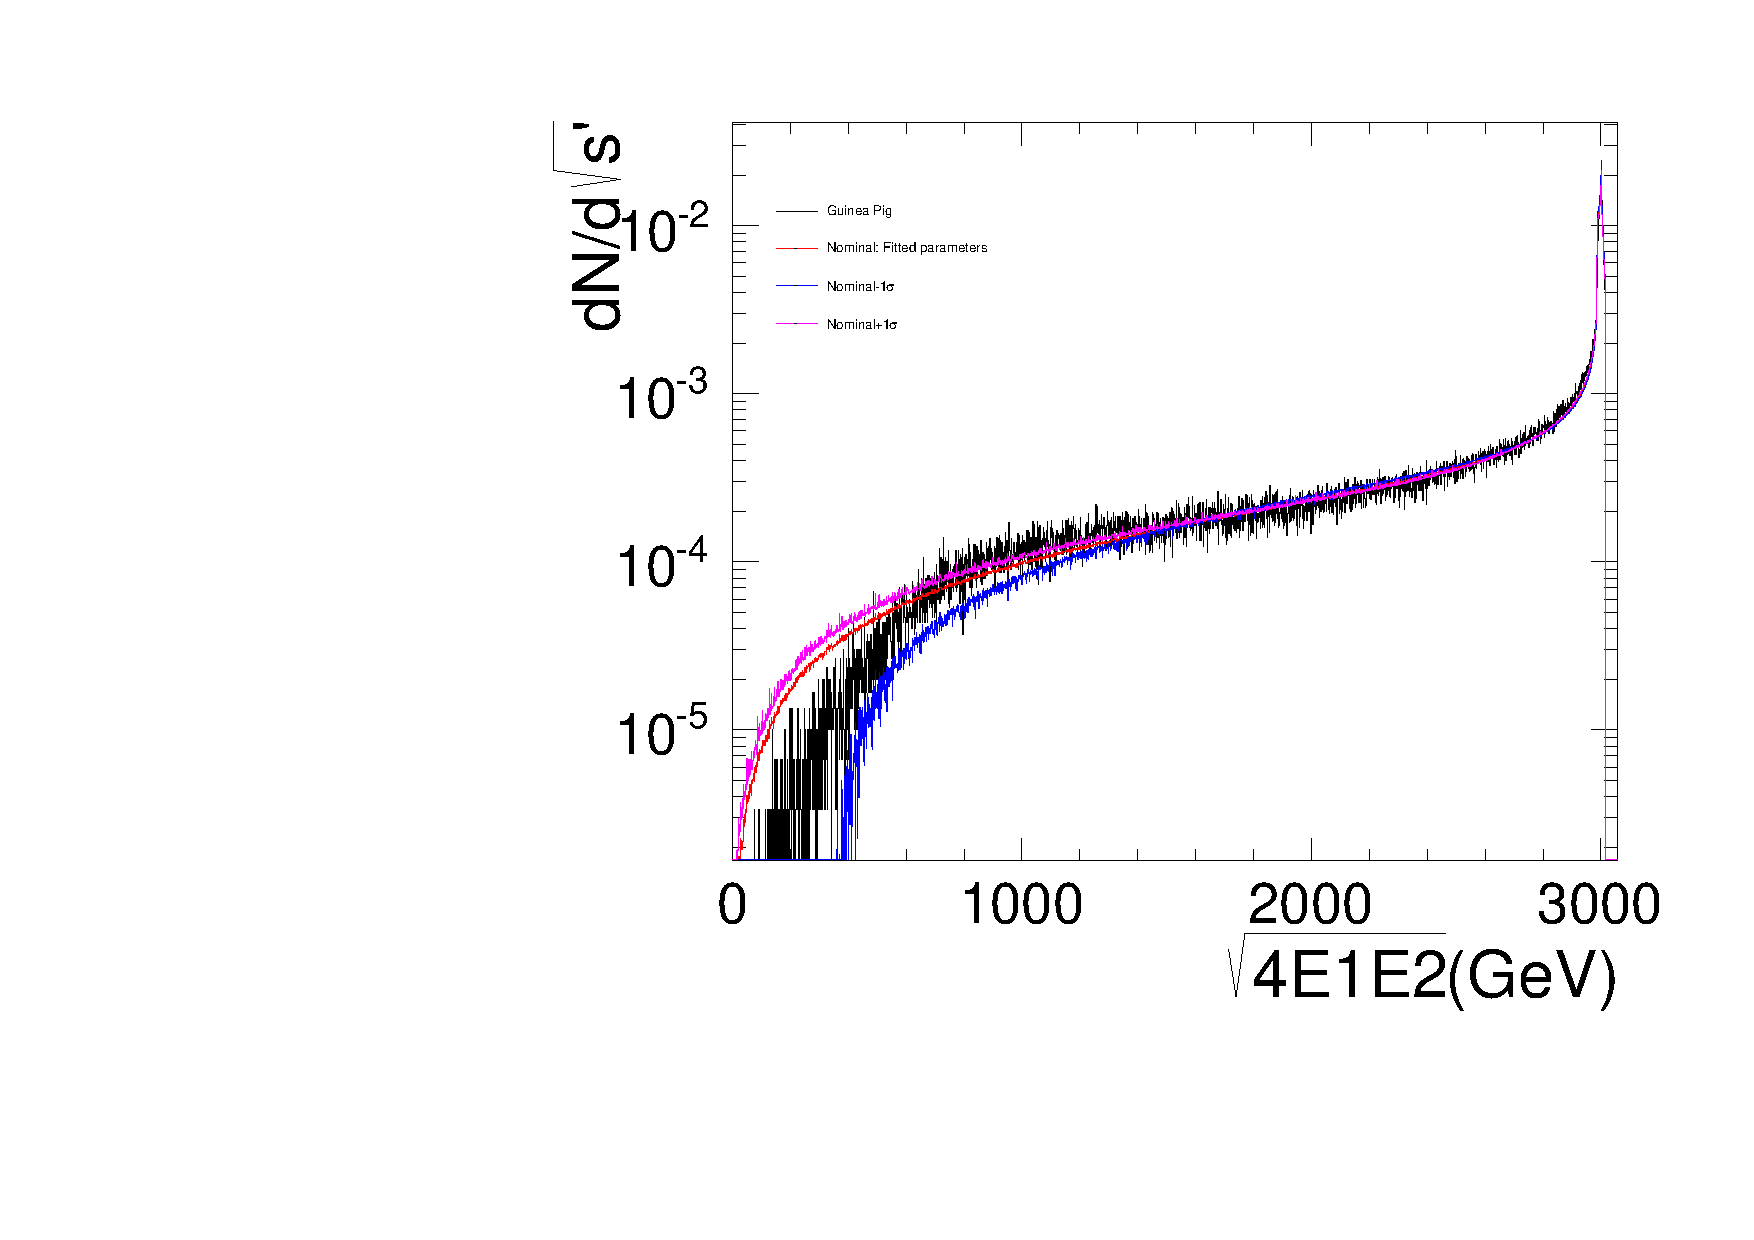
\includegraphics[width=10cm,page=1]{LumiAll.pdf}
\end{center}
\end{frame}
\begin{frame}
\frametitle{Current status: 3e5 events, BHWide, E smeared}
\begin{tikzpicture}
\node[](0.0,-0.3){\includegraphics[width=10cm,clip,page=2]{LumiAll.pdf}};
\coordinate (circ1) at (1.0,0.5);
\draw<2>[line width=0.03cm,color=red](circ1) ellipse(6mm and 10mm);
%\draw<2>[step=0.1,line width=0.001cm,color=green] (0.0,0.0) grid(2,2);
\end{tikzpicture}
\end{frame}
\begin{frame}
\frametitle{Current status: 3e5 events, BHWide, E smeared}
\begin{tikzpicture}
\node[](0.0,-0.3){\includegraphics[width=10cm,page=4]{LumiAll.pdf}};
\coordinate (circ1) at (4.0,-0.5);
\draw<2>[line width=0.03cm,color=red](circ1) ellipse(6mm and 10mm);
\end{tikzpicture}
\end{frame}
\begin{frame}
\frametitle{Current status: 3e5 events, BHWide, E smeared}
\begin{center}
\includegraphics[width=10cm,page=3]{LumiAll.pdf}
\end{center}
\end{frame}
\section{Ideas}
\begin{frame}
\frametitle{Ideas to proceed}
\begin{itemize}
  \item Increase MC statistic used in Fit: reduce stat. fluctuations. Currently
  uses same stat for MC and ``data'': $\sqrt{2}$ factor on every error. By using
  10 times more MC, the error factor drops to $\approx 1.05 \to$ more accurate.
  Running now.
  \item Increase ``data'' statistic: More accurate fit of the tails (later)
  \item Make the 2 ``tails'' share the same parameters: assume them to be
  symetric
\end{itemize}
All this will increase the time needed to obtain a result as the fitting will
take longer
\end{frame}
\section{Conclusion}
\begin{frame}
\frametitle{Conclusion}
\begin{itemize}
  \item Bug found
  \item Current fit results not really better, in particular in the peak region
  \item ``final'' results by the end of the week
  \item Need to write up the procedure for CDR
\end{itemize}
\end{frame}
\end{document}